%______________________________________________________________________
\clearpage
\section*{\centering A Case Study for Grain Quality Assurance Tracking based on a Blockchain Business Network}
%______________________________________________________________________

\subsection*{Authors}
The authors of the paper \cite{2018_Lucena} can be viewed in table \ref{tab:2018_Lucena_Authors}.
\begin{longtable}{ |P{3cm}|P{4cm}|P{5cm}| }
	\caption{Authors} \label{tab:2018_Lucena_Authors} \\
	\hline
 	\cellcolor{Gray}Name & \cellcolor{Gray}Location & \cellcolor{Gray}Institution \\ [0.5ex] 
 	\hline\hline
 	\endhead
 	Percival Lucena & \multirow{2}{4cm}{\centering Brazil}  & \multirow{2}{5cm}{\centering IBM Research\urlfootnote{https://researcher.watson.ibm.com/researcher/view_group_pubs.php?grp=5113}} \\
	\cline{1-1}
	 Alecio P. D. Binotto &   &  \\
	 \hline
	 Fernanda da Silva Momo & Porto Alegre, Brazil  &  Federal University of Rio Grande do Sul (UFRGS) \nomenclature[U]{UFRGS}{Federal University of Rio Grande do Sul}\\
	 \hline
	 Henry Kim & Toronto, Canada  & York University\\
	 \hline
\end{longtable}

%______________________________________________________________________

\subsection*{Contribution}
The contribution of \citet{2018_Lucena} is a grain quality assurance tracking system.
Their work is not available open source. Say here that the system was a real world use case and actually installed and tested in brazil.

%______________________________________________________________________

\subsection*{Reason/Problems}
The brazilian \quoteit{Grain Exports Business Network (GEBN)}\nomenclature[O]{GEBN}{Grain Exports Business Network} is composed of the following actors:
\begin{enumerate}[label={\arabic*)},font={\color{red!50!black}\bfseries},noitemsep]
	\item \textbf{Grain Producer}
	\item \textbf{Rural Credit Bank agent}
	\item \textbf{Private warehouse agent}
	\item \textbf{Trading company agent}
	\item \textbf{Food processing company}
\end{enumerate}
\begin{figure}[!ht]
    \centering
    \label{fig:2018_Lucena_Implementation_Business}
    \caption{Business Network}
    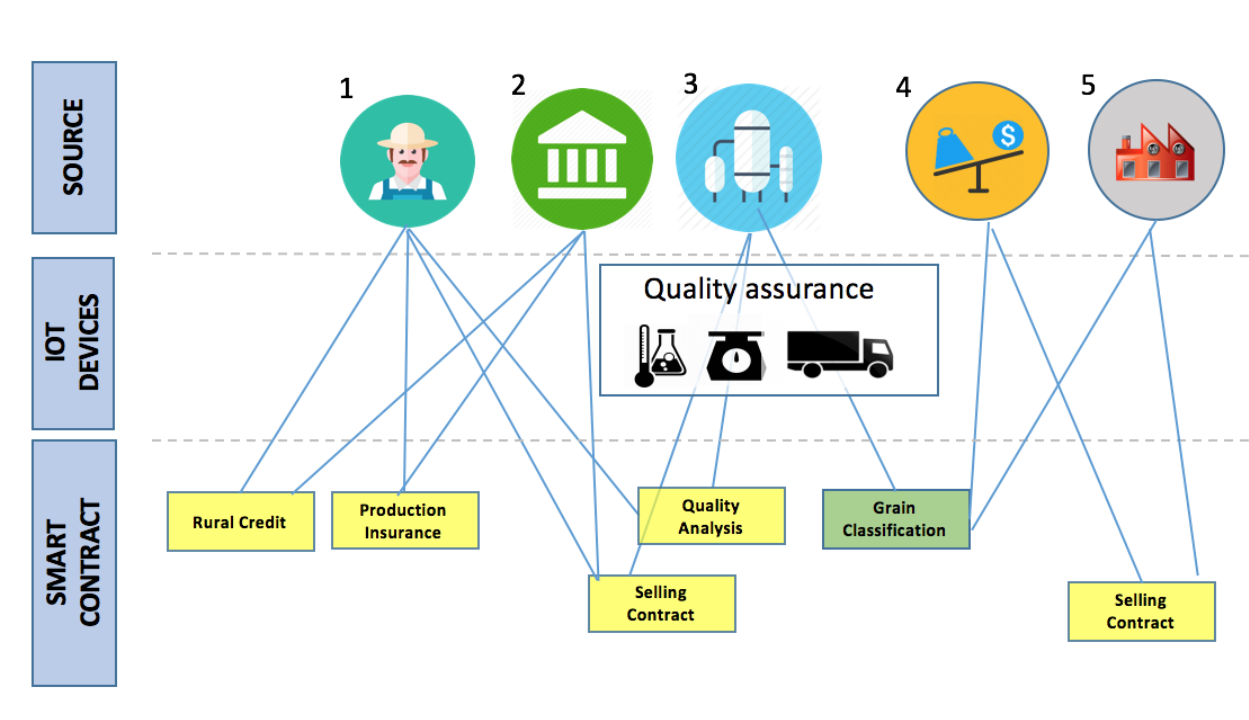
\includegraphics[width=0.8\textwidth]{2018_Lucena_1.png}
\end{figure}
The actors in the GEBN network are not able to trust in each other, because they all have different business goals. This leads to various problems in logisitics and information manangement.\\
In lgoistics, the main problem is:
\begin{enumerate}[label={\arabic*)},font={\color{red!50!black}\bfseries},noitemsep]
	\item There a tremendous logistics and warehouse issues in the moving process of the production from the fields to the other actors on the supply chain. The transportation network and warehouse storage method today has a huge influence on the grain quality.
\end{enumerate}
Since there is no trust, the actors are not willing to share their information with the others. This resolves in multiple problems:
\begin{enumerate}[label={\arabic*)},font={\color{red!50!black}\bfseries},noitemsep]
	\item The grain quality control information is saved in various software programs and then distributed to diverse databases. This leads to inaccurate information flow which causes financial losses in the agreement process between producers and traders.
	\item  Also the real time information about the grain quality is only available to the local actor and not shared with all other players on the supply chain.
\end{enumerate}

Each of these actors has his own issues with the way the current system works.  In the table \ref{tab:2018_Lucena_concerns}, an overview of all actors are listed with their concern and the reason why they have it.
\begin{longtable}{ |P{3cm}|P{4cm}|P{5cm}| }
	\caption{Issues with current network} \label{tab:2018_Lucena_concerns} \\
	\hline
 	\cellcolor{Gray}Actor & \cellcolor{Gray}Concern & \cellcolor{Gray}Reason \\ [0.5ex] 
 	\hline\hline
 	\endhead
	\multirow{3}{3cm}{\centering Grain Producer} & Correct management of grain ingest and classification & Receive a fair payment \\
	\cline{2-3}
	 & \multirow{2}{4cm}{\centering Proper ingest receipt} & Acquire a credit on Rural Credit Banks\\
	 \cline{3-3}
	 & & Agree on a production insurance \\
	 \hline
	 Rural Credit Bank agent & \multirow{2}{4cm}{\centering Accurate data from producers} & Lower credit giving risks\\
	 \cline{3-3}
	 & & Offer reduced interest credit rates for credit operations\\
	 \hline
	 Private Warehouse agent & Precise grain classification data & Sell the grains to various actors \\
	 \hline
	 Trading Company agent & Purchase of large amounts of grains with the right quality from several warehouses & Achieve an export request \\
	 \hline
	 Food processing company & Acquisition of special selected grains that have specific characteristics (e.g.\ high protein) & \xmark \\
	 \hline
\end{longtable}

%______________________________________________________________________

\subsection*{Implementation Process}
To implement their prototype, they used the permissioned Blockchain \quoteit{Hyperledger Farbic Blockchain V1}. There are multiple distributions of this product and they used a cloud instance. Another IBM product they used is the Hyperledger Composer Framework for the creation of smart contracts. The hyperledger framework is hosted on the IBM cloud. Via a Node.js, the system then communicates with the \quoteit{Grain Controller Desktop Application (GDPA)}.\\
The protoype was actually tested in a warehouse in Brazil. The grain quality was tested and then the information about it was documented onto the Blockchain. 


\begin{figure}[!ht]
    \centering
    \label{fig:2018_Lucena_Implementation_Architecture}
    \caption{Architecture}
    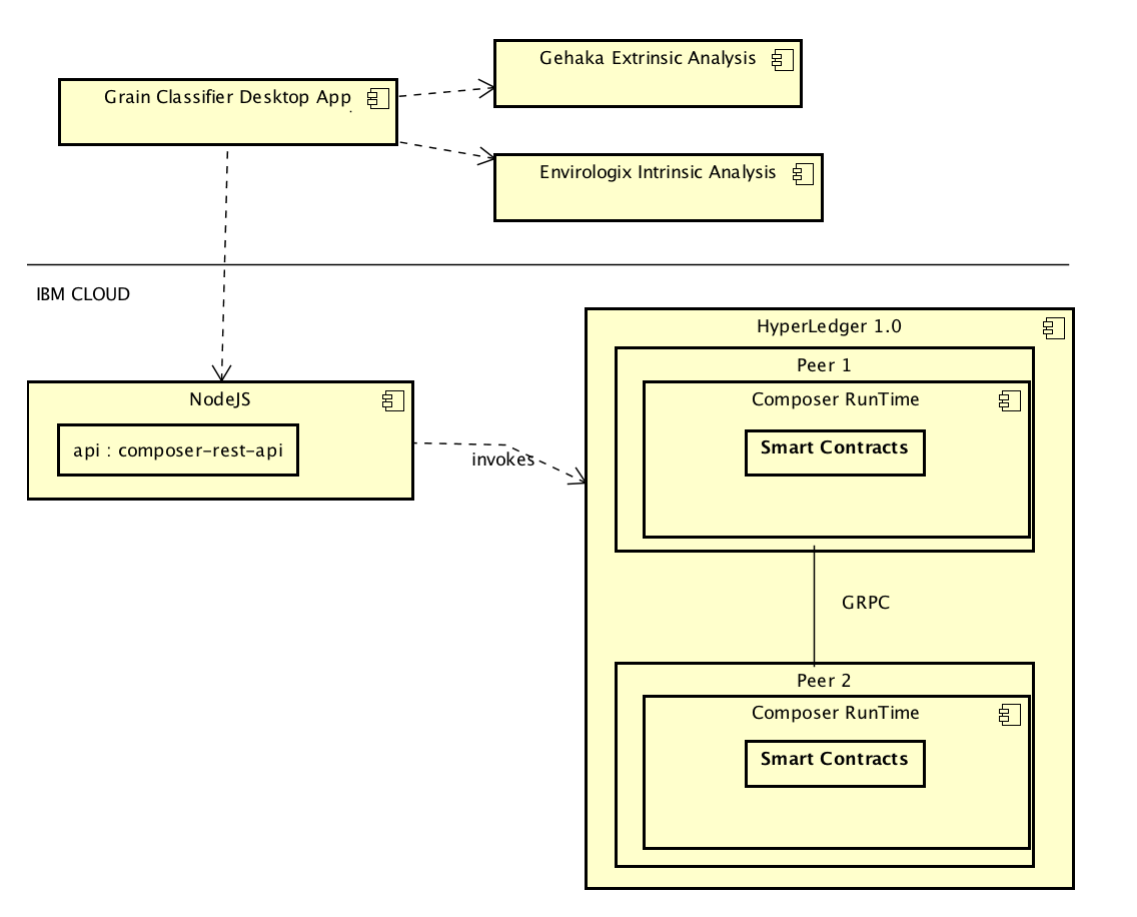
\includegraphics[width=0.8\textwidth]{2018_Lucena_2.png}
\end{figure}
%______________________________________________________________________

\subsection*{Conclusion}
The main benefits of using a Blockchain in this scenario are:
\begin{enumerate}[label={\arabic*)},font={\color{red!50!black}\bfseries},noitemsep]
	\item All members of the supply chain can now use the same business rules and also share the same transaction data. This lowers the discussions between business partners.
	\item Since the Blockchain is very transparent, the participating actors are forced to collaborate with each other to define common rules for the smart contracts. This provides them with the opportunity to define or even vote on their own common rules and consensus principles.
\end{enumerate}
They also mention that in this area, there is future work to do.\\
Especially, they discuss the legal value that is offered with the Blockchain. In this case, Brazil excepts these digital signatures as a valid legal contract. Unfortunately, this is more difficult for a more international solution and yet to prove.\\
Also they state that Blockchain could be a huge advantage for Global Trade. All partner that trade can share their information on a Blockchain and therefore avoid large paper trails and information loss.\\
Overall their project was succesfull and they encourage others to future explore Blockchain Business Networks in other industries.